\documentclass[a4paper,11pt,twoside]{report}
\usepackage{bftn}
\usepackage{calc}
\usepackage{hyperref}
\usepackage{hyphenat}
\usepackage{verbatim}
\usepackage{xspace}
\usepackage{pifont}
\usepackage{pxfonts}
\usepackage{textcomp}
\usepackage{amsmath}
\usepackage{listings}
\usepackage[framemethod=default]{mdframed}
\usepackage[shortlabels]{enumitem}
\usepackage{parskip}
\usepackage{xparse}
\usepackage{natbib}
\usepackage[all,cmtip]{xy}
\usepackage{xcolor}% or package color

\title{Device Queues in Barrelfish}
\author{Barrelfish project}
\tnnumber{26}
\tnkey{DeviceQueues}

\begin{document}
	\maketitle			% Uncomment for final draft
	
	\begin{versionhistory}
		\vhEntry{0.1}{24.10.2017}{RH}{Initial Version}
	\end{versionhistory}
	
	% \intro{Abstract}		% Insert abstract here
	% \intro{Acknowledgements}	% Uncomment (if needed) for acknowledgements
	\tableofcontents		% Uncomment (if needed) for final draft
	% \listoffigures		% Uncomment (if needed) for final draft
	% \listoftables			% Uncomment (if needed) for final draft
	\cleardoublepage
	\setcounter{secnumdepth}{2}

	\newcommand{\todo}[1]{[\textcolor{red}{\emph{#1}}]}

	\newcommand{\virtio}{Virtio }
	\newcommand{\devif}{Devif }
	\newcommand{\ep}[1]{$Ep_{#1}$}

\usepackage{color}
\definecolor{bluekeywords}{rgb}{0.13,0.13,1}
\definecolor{greencomments}{rgb}{0,0.5,0}
\definecolor{redstrings}{rgb}{0.9,0,0}

\lstdefinestyle{code}
{language=C,
	basicstyle=\tiny,
	showspaces=false,
	showtabs=false,
	breaklines=true,
	showstringspaces=false,
	breakatwhitespace=true,
	escapeinside={(*@}{@*)},
	commentstyle=\color{greencomments},
	keywordstyle=\color{bluekeywords}\bfseries,
	stringstyle=\color{redstrings},
	basicstyle=\ttfamily,
	morekeywords={uint8_t, uint16_t, uint32_t, uint64_t, size_t, bool},}
	
	\mdfdefinestyle{defi}{%
		linecolor=black,linewidth=2pt,%
		frametitlerule=true,%
		frametitlebackgroundcolor=gray!20,
		innertopmargin=\topskip,
		nobreak=true% prevent page breaks in the middle of mystyle
	}
	
	\mdfdefinestyle{inv}{%
		linecolor=black,linewidth=2pt,%
		topline=false,
		leftline=false,
		innertopmargin=\topskip,
	}
	
	\mdtheorem[style=defi]{defi}{Definition}
	\mdtheorem[style=defi]{op}{Operation}
	\mdtheorem[style=inv]{inv}{Invariant}
	
	\chapter{Introduction}
	In this document we describe a queue based interface that unifies communication for 
	devices like network cards and block devices but also between processes. 
	The interface should fit to as many devices as possible while still being efficient.
	The goal is similar to \virtio \cite{virtio:sigops}, Portals \cite{portals} or MPI \cite{mpi}, 
	but we want to take a more formal 
	approach and define pieces that are ambiguous. These interface do not define a memory model 
	or what preconditions/postconditions an interface function has. 
	For example, what happens when a guest accesses a memory buffer that is handed off 
	to the host? These interfaces are clearly implementation driven where 
	we want to document the interface as clearly as possible, and see the implementation and
	its code as two separate things.
	
	\section{Terminology}
	In this section, we explain the terms and the meaning of them as they are used in the following sections.
	\begin{itemize}
		
		\item \textbf{Region}: A Region is a chunk of memory that is registered to the \devif interface. From the memory of the region, buffers can be allocated.
		\item \textbf{Buffer}: A buffer is a chunk of memory within a region.
		\item \textbf{Endpoint}: An endpoint is a processes or devices. 
		\item \textbf{Ownership}: An endpoint can own a buffer and transfer ownership of a buffer to another endpoint or device. 
		If an endpoint owns a buffer, it can alter it. If an endpoint alters a buffer that is not owned, 
		the result is undefined and it is considered a bug. 
	\end{itemize}
	
	\section{Functionality}
	The basic functionality of our queue based device interface (from now on called \devif) 
	should be transferring ownership of buffers between two endpoints of a queue.  
	A buffer is a variable sized piece of memory within a previously to the \devif interface 
	register region of memory. We exclude managing the buffers themselves i.e. allocating 
	and deallocating buffers to keep the interface and the underlying protocol simple. 
	If we manage the variable sized buffers, we would have to implement a dynamic memory 
	allocator which increases the complexity of the \devif interface. 
	\\
	Another important aspect is the idea of "stacking" queues. In this manner each 
	queue on the stack can do an arbitrary transformation on the buffer that was enqueued 
	and hand it down to the queue lower in the stack. 
	
	\section{Memory Model}
	When implementing a backend for the \devif interface, the underlying memory model 
	has to be considered. In certain cases, a write to a buffer might not have been written back
	to memory before the buffer is processed by a device. 
	\\
	There are several memory models that are used in current hardware but none of them 
	are sequential consistent (SC). The memory models relax sequential consistency to allow 
	instruction reordering and other optimizations. Currently X86 and Sparc can be 
	modelled using \textit{Total Store Ordering} (TSO) ~\cite{swell:cacm2010}. TSO relaxes 
	SC so that local writes are visible locally before they are visible to all other
	hardware threads (multi-copy atomic). In most cases this is because of a write buffer
	that is introduced to buffer stores and the local request are satisfied by the contents 
	of the buffer. TSO is still a very strict memory model and only allows limited instruction
	reordering. 
	\\
	Our aim with \devif is that the backends support the even more relaxed model of ARM 
	\cite{swell:cacm2016,arm:mm} (and IBM Power). In the memory model of ARM the processor can 
	reorder instructions very generously. Stores as well as loads and other instructions 
	(even atomic instructions) can be reordered. The goal of \devif is to support the weakest memory
	model so it runs on the most common hardware, but can still increase the strictness
	of the memory model to improve performance. 
	

	\chapter{Function Definitions and Semantics}
	In this section we describe the functions of the \devif interface in detail. 
	Not only do we define the functions itself, 
	but the give additional information to the semantics. We use the term 
	\textit{undefined behaviour} for calls on the interface that we consider
	bugs and that must not happen. The creation and destruction of queues 
	are device specific and are not part of the interface itself. 
	
	\section{Registering Region}
	Adds a region of memory to the active set of this queue. 
	The queue has to be properly initialized beforehand. 
	The memory region has to be owned by the endpoint trying to register the region. 
	If the region is not owned by the endpoint, the behaviour is undefined.
	If a region is added that is already registered or overlaps with another region, an error must be returned. 
	The returned region id must be unique for this queue and larger than or equal to 0. After the function returns, 
	buffers from the just registered region can be enqueued and the ownership
	can be transferred. 
	\begin{figure}[h]
		\begin{lstlisting}[style=code]
        errval_t devq_register(struct devq *q,
                               struct capref cap,
                               regionid_t* region_id);
		\end{lstlisting}
		\label{lst:register}
	\end{figure}
	
	\subsection*{Arguments}
	\begin{itemize}
		\item \texttt{devq *q}: handle to the device queue.
		\item \texttt{struct capref cap}: the capability representing the memory region to register.
		\item \texttt{regionid\_t* region}: return pointer to the region id of the newly registered region.
	\end{itemize}
	\subsection*{Preconditions}
	\begin{itemize}
		\item The device queue is initialized
		\item The memory has to be allocated
		\item Memory of the region must be owned by endpoint 
		\item The region must not be currently registered
		\item Region must not overlap with other already registered regions 
	\end{itemize}
	\subsection*{Postconditions}
	On success, the following conditions on the returned value hold
	\begin{itemize}
		\item \texttt{region\_id} must be unique for this queue and larger or equal to 0
	\end{itemize}
	
	\subsection*{Reasons for Failure}
	\begin{itemize}
		\item Register function of backend fails.
		\item Region to register is already registered.
	\end{itemize}
	
	\section{Deregister Region}
	Removes a memory region from the registered regions of a queue. 
	If a region is deregisterd that was not registered before, an error is returned. 
	To deregister a region, every buffer of the region i.e. the whole region has to be 
	owned by the endpoint making the call to the interface. If a region is deregistered and the 
	region is not fully owned by the endpoint, the behaviour is undefined.  
	\begin{figure}[h]
		\begin{lstlisting}[style=code]
        errval_t devq_deregister(struct devq *q,
                                 regionid_t region_id,
                                 struct capref* cap);
		\end{lstlisting}
		\label{lst:deregister}
	\end{figure}
	
	\subsection*{Arguments}
	\begin{itemize}
		\item \texttt{devq *q}: handle to the device queue
		\item \texttt{regionid\_t region\_id}: the id of the region to deregister
		\item \texttt{struct capref cap}: return pointer to the cap of the deregistered region
	\end{itemize}
	
	\subsection*{Preconditions}
	\begin{itemize}
		\item The device queue is initialized
		\item Region must currently be registered (i.e. valid region id that is currently registered)
	\end{itemize}
	\subsubsection*{Postconditions}
	On success, the following conditions on the returned value hold
	\begin{itemize}
		\item \texttt{cap} must not be NULL
		\item \texttt{cap} is a capability referencing a memory region that was once registered.
	\end{itemize}
	
	\subsection*{Reasons for Failure}
	\begin{itemize}
		\item Backend deregister function fails.
		\item Region was not registered beforehand. 
	\end{itemize}
	
	\section{Enqueue}
	Enqueues a buffer of a region for ownership transfer. The buffers offset into the memory region 
	has to be within the preregistered memory region matching the region id, otherwise an error is returned. 
	The region id provided has to be valid i.e. larger or equal than 0 and is already registered. 
	The length of the buffer must be large than 0 and must not
	exceed the region size minus the offset of the start address of the buffer within the 
	region. The valid data offset has to be within the buffer and its length may not exceed
	the buffers length. 
	The buffer has to be currently owned by the client i.e. a buffer 
	can not be enqueued twice without dequeuing it beforehand, otherwise the behaviour is undefined. 
	Enqueueing a buffer does not directly transfer the ownership, but the client
	enqueueing the buffer has given up ownership on the buffer. Eventually the ownership
	of the buffer will be transferred but there is no guarantee when this happens.
	All the changes to the buffer have to be written back to memory and not only 
	reside in the cache. Altering a buffer that a client has no ownership over, 
	will result in undefined behaviour. Multiple buffers can be chained by using 
	the argument \texttt{misc\_flags}. When chaining multiple buffers, the last buffer
	of the chain must have the \texttt{misc\_flags} set to \texttt{DEVQ\_FLAG\_LAST}.
	
	
	\begin{figure}[h]
		\begin{lstlisting}[style=code]
		errval_t devq_enqueue(struct devq *q,
		                      regionid_t region_id,
		                      genoffset_t offset,
		                      genoffset_t length,
		                      genoffset_t valid_data,
		                      genoffset_t valid_length,
		                      uint64_t misc_flags);
		\end{lstlisting}
		\label{lst:enqueue}
	\end{figure}
	
	\subsection*{Arguments}
	\begin{itemize}
		\item \texttt{devq *q}: handle to the device queue.
		\item \texttt{regionid\_t region\_id}: the id of a memory region the enqueued buffer belongs to.
		\item \texttt{genoffset\_t offset}: the offset within the memory region where the buffers starts. 
		\item \texttt{genoffset\_t length}: the length of the enqueued buffer.
		\item \texttt{genoffset\_t valid\_data}: the offset within the buffer where the valid data starts.
		\item \texttt{genoffset\_t valid\_length}: the length of the valid data within the buffer.
		\item \texttt{uint64\_t flags}: flags of the buffer. 
	\end{itemize}
	
	\subsection*{Preconditions}
	\begin{itemize}
		\item The device queue is initialized
		\item The region id must match with an already registered region
		\item The buffer must be owned by the client of the interface 
		\item The offset must be within the bounds of a memory region
		\item The length must not exceed the region size minus the offset of the buffer within the region
		\item The valid\_data offset must be within the buffers bounds
		\item The valid\_length must not exceed the length minus the valid\_data offset
		\item Changes to the buffer are written back to memory
	\end{itemize}
	
	\subsection*{Postconditions}
	After a successful enqueue, the following conditions hold
	\begin{itemize}
		\item -
	\end{itemize}
	
	\subsection*{Reasons for Failure}
	\begin{itemize}
		\item Backend enqueue function fails (e.g. when the queue is full)
		\item Region id is not valid.
		\item Bounds check for buffer fails
		\item Bounds check for valid data fails
	\end{itemize}
	
	\section{Dequeue}
	Dequeues a buffer from the queue. After a buffer is dequeued, the client
	takes ownership of the buffer. As long as the client owns a buffer, the
	client can alter the contents of this buffer. Dequeue can be called any time,
	and even when a notification is received there is no guarantee that the queue contains any buffers
	to receive. If there is nothing to dequeue, the call will return an error. When an endpoint
	dequeues a buffer, it has to invalidate its cache of the received buffer when
	the weaker memory model is assumed (ARM, IBM Power). The dequeued values 
	have to represent a valid buffer as well as point to valid data. If nothing 
	is known about the validity of the data with the buffer, the whole buffer 
	is considered as valid data.

	\begin{figure}[h]
		\begin{lstlisting}[style=code]
		errval_t devq_dequeue(struct devq *q,
		                      regionid_t* region_id,
		                      genoffset_t* offset,
		                      genoffset_t* length,
		                      genoffset_t* valid_data,
		                      genoffset_t* valid_length,
		                      uint64_t* flags);
		\end{lstlisting}
		\label{lst:dequeue}
	\end{figure}
	\subsection*{Arguments}
	\begin{itemize}
		\item \texttt{devq *q}: handle to the device queue.
		\item \texttt{regionid\_t* region\_id}: return pointer to the region id of the dequeued buffer.
		\item \texttt{genoffset\_t* offset}: return pointer to the offset within the memory region where the buffers starts. 
		\item \texttt{genoffset\_t* length}: return pointer to the length of the enqueued buffer.
		\item \texttt{genoffset\_t* valid\_data}: return pointer to the offset within the buffer where the valid data starts.
		\item \texttt{genoffset\_t* valid\_length}: return pointer to the length of the valid data within the buffer.
		\item \texttt{uint64\_t flags}: flags of the buffer. 
	\end{itemize}
	\subsection*{Preconditions}
	\begin{itemize}
		\item The device queue is initialized
	\end{itemize}
	\subsection*{Postconditions}
	The returned pointer have to contain valid information about a buffer.
	After a successful dequeue, the following conditions on the returned values hold
	\begin{itemize}
		\item \texttt{region\_id} must be larger or equal to 0
		\item \texttt{offset} is not equal to \textit{NULL}
		\item \texttt{length} is not equal to \textit{NULL}
		\item \texttt{valid\_data} is not equal to \textit{NULL}
		\item \texttt{valid\_length} is not equal to \textit{NULL}
		\item \textit{offset} does not exceed region length
		\item \textit{length} + \textit{offset} do not exceed region length
		\item \textit{valid\_data} does not exceed the buffer size
		\item \textit{valid\_length} does not exceed buffer size minus valid data offset
	\end{itemize}
	
	\subsection*{Reasons for Failure}
	\begin{itemize}
		\item Backend dequeue function fails (e.g. when the queue is empty)
		\item Buffer returned by the backend is not valid.
	\end{itemize}
	
	\section{Notify}
	Notify informs the client on the other side of the queue that there might be buffers 
	buffers in the queue that are ready for processing. There is no guarantee that there is 
	actually a buffer in the queue. When a buffer is enqueued, there
	is no guarantee to when the buffer is processed. Notify ensures, that
	all the buffers that are enqueued to this point will eventually processed and the ownership
	is transferred. Notify is a performance optimization mechanism and not strictly necessary.
	
	\begin{figure}[h]
		\begin{lstlisting}[style=code]
		errval_t devq_notify(struct devq *q);
		\end{lstlisting}
		\label{lst:notify}
	\end{figure}
	
	\subsection*{Arguments}
	\begin{itemize}
		\item \texttt{devq *q}: handle to the device queue.
	\end{itemize}
	\subsection*{Preconditions}
	\begin{itemize}
		\item The device queue is initialized
	\end{itemize}
	\subsection*{Postconditions}
	-- 
	\subsection*{Reasons for Failure}
	\begin{itemize}
		\item Backend notify function fails
	\end{itemize} 
	
	\chapter{Formal Model}
	In this section we model the system as a transfer of ownership of sets of addresses. We model it as a 
	transition system by first defining the agents, the structures, 
	and the operations used to do the transfer. We do not model notifications since they are strictly optional
	and mainly a performance optimization. We abstract the buffers 
	of the ownership transfer protocol as a simple set of addresses. Consequently, we do not need to 
	define what a buffer is. This means in our model the smallest unit resource we transfer ownership 
	of is a single memory address. 
	\\
	\begin{defi}[Memory Address]
		A \textbf{Memory Address} \textit{A} is an identifier (or a name) that abstracts 
		an addressable byte of a machine. 
	\end{defi}
	
	To go any further, we have to define on what sets an agent can operate on. In the following
	if we write about a set, this means a set of addresses i.e. if we mention set $S$ it 
	is defined as $S = \{A_0, ..., A_n\}$.
    In our transition system we only have two agents $X$ and $Y$.
	\\
	\begin{defi}[Agent State]
		Our model consists of two Agents $X$ and $Y$. 
		The sets an Agent can operate on are $S_x$ for agent $X$ and $S_y$ for agent $Y$ and
		each of these sets consists of memory addresses.
	\end{defi}
	
	The ownership in our model is transferred between the two agents $X$ and $Y$. 
	If an agent takes ownership of an address, this means that the agent can operate 
	on these addresses. For example, it can read the 
	contents of the memory address or write to the memory address. 
	\\
	\begin{defi}[Ownership]	
		Agent $X$ and $Y$ can take \textbf{ownership} of an address $A$ by adding the memory address to the set $S_x$ or $S_y$ respectively.
		\[ \text{ownership}(S, A) \Leftrightarrow A \in S \] 
		where $S$ is either the state of agent $X$ or $Y$ and $A$ is any address that can be used in the transition system. 
	\end{defi}
	
	To prevent two agents owning the same address, we define the following invariant that 
	has to hold for all operations on the transition system.
	\\
	\begin{inv}
		At any point in time an address $A$ can only be owned by one Agent at a time
		\[ S_x \cap S_y = \emptyset \]
	\end{inv}	
	
	With the current definitions, we could model the transfer of ownership by simply removing from one
	set and adding it to the other ($S_x$ to $S_y$ and vice versa) but this model would not 
	entail correctly how the transfer of an address happens. An address that is enqueued might
	not be immediately dequeued by the other agent which means that we require another mechanism: 
	the queue itself. In essence, we need to store
	the addresses that are currently in transfer in another set associated with a queue.
	\\
	\begin{defi}[Queue]
		A bidirectional queue $Q$ between the two agents $X$ and $Y$ consists of two sets of addresses called 
		$T_{xy}$ and $T_{yx}$ where $T_{xy}$ is the set of addresses that is in transfer from agent $X$ 
		to agent $Y$ and $T_{yx}$ vice versa. 
		\[Q = (T_{xy}, T_{yx})\]
	\end{defi}
	
	Having defined basic agents and structures of our model, but we are missing operations 
	on the transition system to actually transfer the ownership of addresses. To transfer 
	ownership over a queue from agent $X$ to $Y$ and vice versa, we define
	the operations \textit{enqueue} and \textit{dequeue}. 
	\\
	\begin{op} [Enqueue]
		Enqueue: initiates a transfer of ownership of a set of addresses $B$ from agent $X$ to $Y$ and vice versa. 
		Enqueue removes $B$ from either agent $X$ or $Y$'s state ($S_x$ and $S_y$) and adds it to the 
		queue $Q$ ($Q.T_{xy}$ in case of agent $X$ and $Q.T_{yx}$ in case of agent $Y$). Enqueue requires a 
		set of addresses to transfer $B$. The function enqueue from agent $X$ is defined as
		\begin{align*} enqueue_{x}(B) \quad \quad S_x := S_x - B \\
		T_{xy} := T_{xy} \cup B  
		\end{align*}
		and for Agent $Y$
		\begin{align*} enqueue_{y}(B) \quad \quad S_y := S_y - B \\
		T_{yx} := T_{yx} \cup B 
		\end{align*}
	\end{op}
	\\
	\\
	\begin{op}[Dequeue]
		Dequeue: completes a transfer of ownership of a set of addresses $B$ from agent $X$ to $Y$ 
		and vice versa. Dequeue removes $B$ from the queue state $Q$ ($Q.T_{xy}$ in case of $Y$ 
		and $Q.T_{yx}$ in case of $X$) and adds it to the agents state $S$ ($S_x$ in case of $X$ and 
		$S_y$ in case of $Y$). Dequeue requires the set of addresses to transfer $B$, the agents state 
		$S$ and the queue state $Q$. The function enqueue from agent $X$ is defined as
		\begin{align*} \text{dequeue}_{x}(B) \quad \quad T_{yx} := T_{yx} - B \\
		S_x := S_x \cup B  
		\end{align*}
		and for Agent $Y$
		\begin{align*} \text{dequeue}_{y}(B) \quad \quad T_{xy} := T_{xy} - B \\
		S_y := S_y \cup B  
		\end{align*}
	\end{op}
	\\
	\\
	Further to add and remove Addresses from the closed system, we defined \textit{register} and \textit{deregister}.
	\begin{op} [Register]
		Register: adds a set of addresses $R$ that are not yet in the system to the agent state $S$. 
		To be more precise $R$ is defined as \[ R \subseteq (S_x \cup S_y \cup Q.T_{xy} \cup Q.T_{yx})^c \]
		
		The addresses in the system can be used for the transfer of ownership to a second agent. 
		The function takes the set of addresses $R$ as an argument
		
		The behaviour of the function \textit{register} is shown below 
		$$register_{x}(R) \quad \quad S_x := S_x \cup R $$
		$$register_{y}(R) \quad \quad S_y := S_y \cup R $$
	\end{op}
	\\
	\vspace{6mm}
	\\
	\begin{op} [Deregister]
		Deregister: removes a set of memory addresses $R$ from an agents
		state $S$. After deregistering the addresses of $R$ can no longer be transfer on
		the queue. The function takes the set of addresses $R$. The addresses
		of $R$ will be no longer in the system i.e. 
		\[R \in (S_x \cup S_y \cup Q.T_{xy} \cup Q.T_{yx})^c \]
		
		The behaviour of the function \textit{deregister} is shown below 
		$$deregister_{x}(R) \quad \quad S_x := S_x - R $$
		$$deregister_{y}(R) \quad \quad S_y := S_y - R $$
	\end{op}
	\clearpage
	The transition system that we defined up to now can be seen in the picture below. 
	
\begin{figure}[!h]
	\begin{center}
		\caption{Buffer transfer protocol sets and the operations}
		\centerline{\xymatrix{
				&&(S_x \cup S_y \cup T_{xy} \cup T_{yx})^c 
				\ar@{<->}[rrddd]^{register_y}_{deregister_y}
				\ar@{<->}[llddd]^{deregister_x}_{register_x}
				\\
				\\
				&&T_{xy} \ar@{->}[rrd]^{dequeue_y} \\
				S_x \ar@{->}[rru]^{enqueue_x} 
				&&&&S_y \ar@{->}[lld]^{enqueue_y}\\
				&&T_{yx} \ar@{->}[llu]^{dequeue_x}
			}}
		\end{center}
\end{figure}
		
	The invariant we described before, only captures part of the constraint that we require so we extend it to
	also address the sets $T_{xy}$ and $T_{yx}$.
	
	\begin{inv}
		At any point in time an address $A$ can only be in one set at the tame
		\[ S_x \cap S_y \cap T_{xy} \cap T_{yx} = \emptyset \]
	\end{inv}	

	We can show that this holds for all the operations we defined. We omit the proof in this document.
	The formal specification should make the main concepts of the \devif Interface more clear and 
	remove more ambiguities of the function specifications and semantics of the previous chapter. 


\chapter{Implementation} 

The building blocks of the \devif interface are the different library backends for the devices
and a small generic library implementing the bookkeeping of region and buffer ids. The backend 
libraries implement a few well defined functions that are installed as function pointers
for the generic library during the creation of a queue. Creating and destroying a queue 
is device specific and is not part of the interface between library backends and the 
generic library. A high level overview of how to use the \devif interface is shown in Figure 
\ref{fig:overview}. The creation of a queue yields a handle that contains all the
state for a device queue and as a first member, the general struct for the \devif
queue state. An example of the data structures for a device and the \texttt{devq struct} 
is shown in Figures \ref{lst:sfn5122f}, \ref{lst:devq}, \ref{lst:func_p}.


\begin{figure}[h]
	\centering
	\caption{High level overview}
	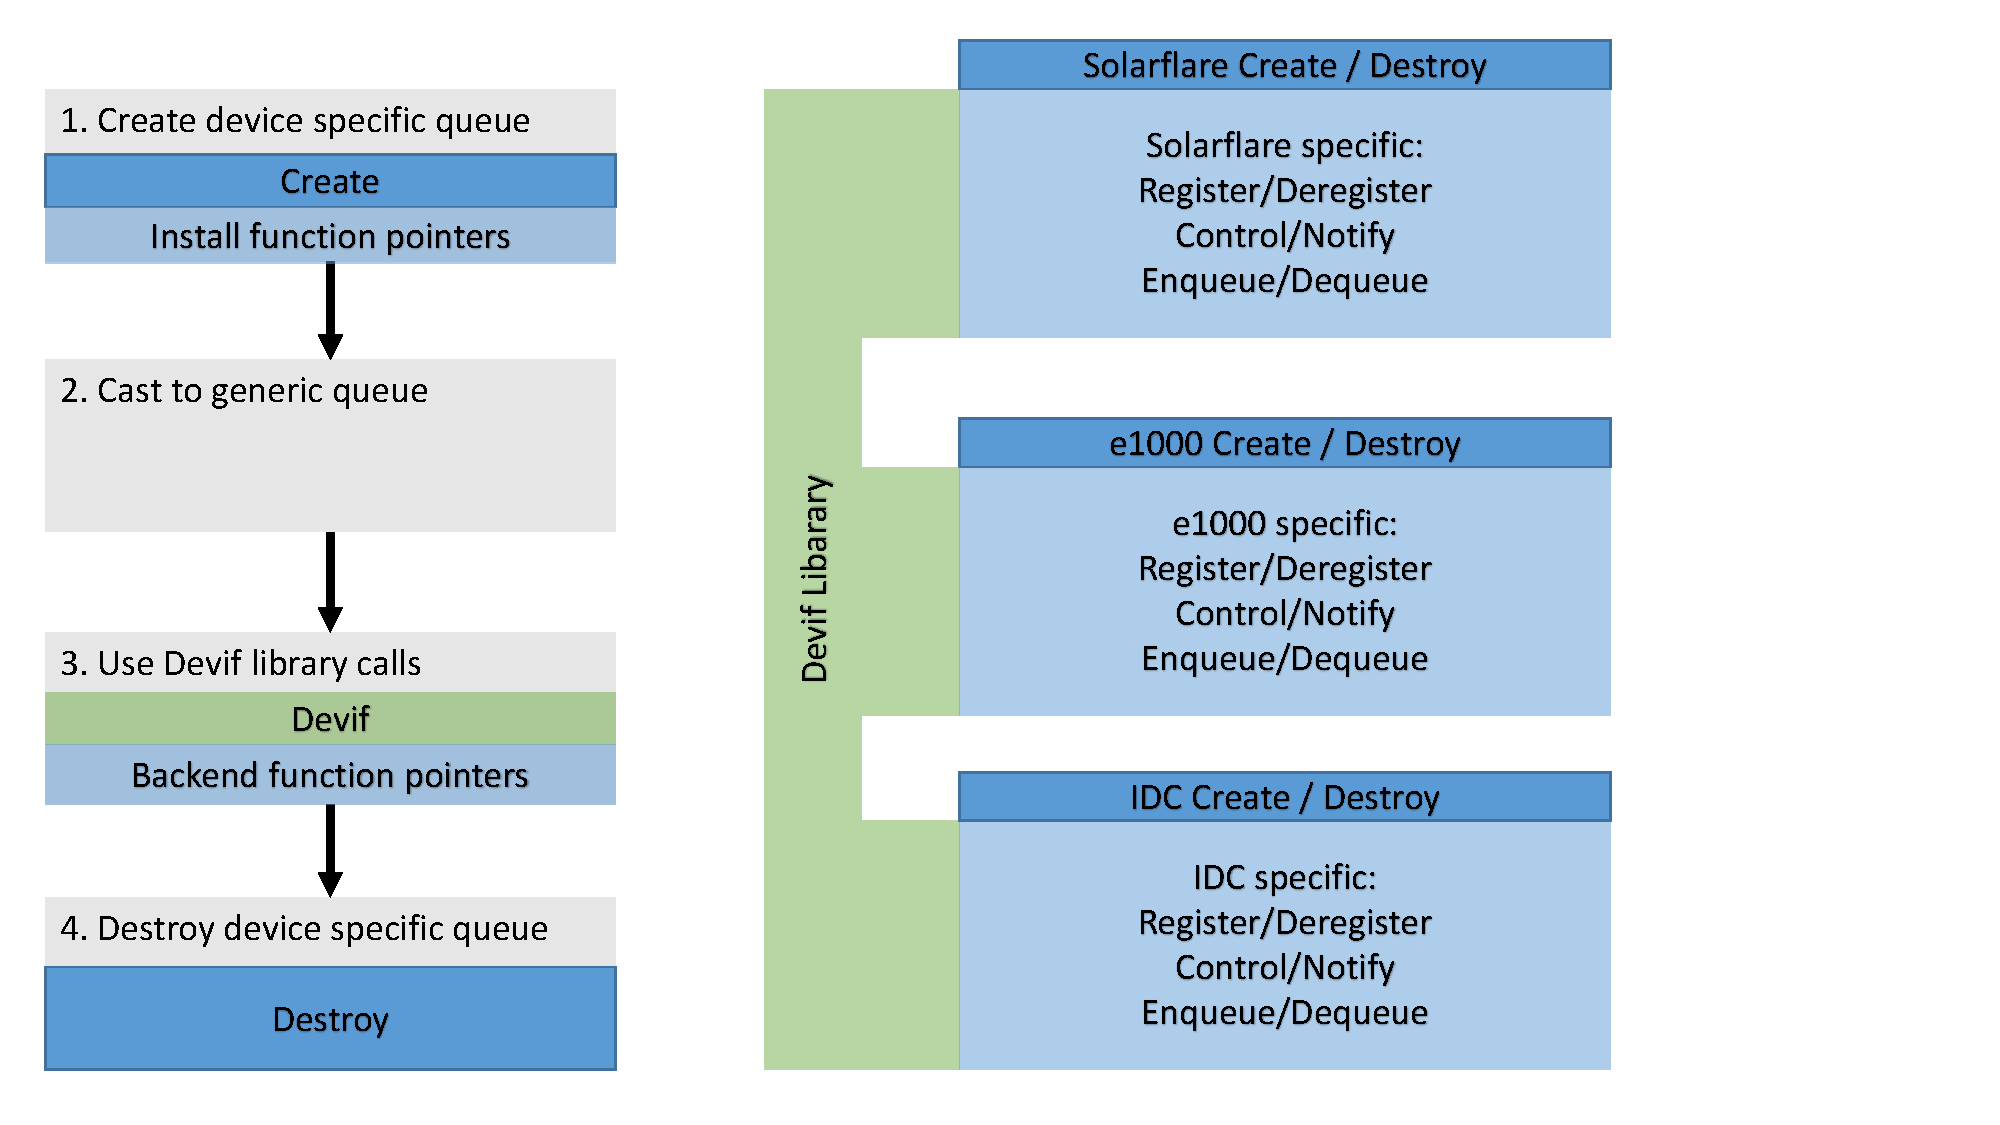
\includegraphics[width=\textwidth]{pics/devif.pdf}
	\label{fig:overview}
\end{figure}  

\begin{figure}[h]
	\caption{Device Specific Queue Struct}
	\begin{lstlisting}[style=code]
    struct sfn5122f_queue {
        struct devq q;
        union {
            sfn5122f_q_tx_user_desc_array_t* user;
            sfn5122f_q_tx_ker_desc_array_t* ker;
        } tx_ring;
        struct devq_buf*                tx_bufs;
        uint16_t                        tx_head;
        uint16_t                        tx_tail;
        size_t                          tx_size;
        ...
    };
	\end{lstlisting}
	\label{lst:sfn5122f}
\end{figure}  

\begin{figure}[h]
	\caption{General \devif struct}
	\begin{lstlisting}[style=code]
    struct devq {
        // Region management
        struct region_pool* pool;
        
        // Funciton pointers
        struct devq_func_pointer f;
        ...
    };
	\end{lstlisting}
	\label{lst:devq}
\end{figure}  

\begin{figure}[H]
	\caption{Backend Function Pointers}
	\begin{lstlisting}[style=code]
    typedef uint64_t genoffset_t;
    errval_t (*devq_notify_t) (struct devq *q);
	
    errval_t (*devq_register_t)(struct devq *q,
                                struct capref cap,
                                regionid_t region_id);
                                
    errval_t (*devq_deregister_t)(struct devq *q, 
                                  regionid_t region_id);
	
    errval_t (*devq_control_t)(struct devq *q,
	                           uint64_t request,
	                           uint64_t value
	                           uint64_t result*);
	
    errval_t (*devq_enqueue_t)(struct devq *q, 
	                           regionid_t region_id,
	                           genoffset_t offset,
	                           genoffset_t length,
	                           genoffset_t valid_data,
	                           genoffset_t valid_offset,
	                           uint64_t misc_flags);
	
    errval_t (*devq_dequeue_t)(struct devq *q,
                               regionid_t* region_id,
                               genoffset_t* offset,
                               genoffset_t* length,
                               genoffset_t* valid_data,
                               genoffset_t* valid_offset,
                               uint64_t* misc_flags);
	
    struct devq_func_pointer {
        devq_register_t reg;
        devq_deregister_t dereg;
        devq_control_t ctrl;
        devq_notify_t notify;
        devq_enqueue_t enq;
        devq_dequeue_t deq;
    };
	\end{lstlisting}
	\label{lst:func_p}
\end{figure}  


The example shown in Figure \ref{lst:sfn5122f} is the device specific struct for a Solarflare NIC queue.
The struct contains as a first member the \texttt{devq} struct (Figure \ref{lst:devq}) so it can be 
cast to a \texttt{devq} struct. The rest of the struct contains the pointers to the descriptor rings (and
the state associated with a descriptor for the \devif interface). Further the bindings for the 
communication channel to the card driver. In Figure \ref{lst:func_p} the functions which have 
to be implemented by a library backend are shown. In certain cases some of these functions
can be a NOP, but the function pointers still have to be set.

\section{Implementation Debug Backend}
This is a debugging interface for \devif interface that            
can be used with any existing queue. It can be stacked on top                
to check for non valid buffer enqueues/deqeues that might happen and
that lead to undefined behaviour. With other queues, the undefined behaviour
might go unnoticed where the debug queue certainly returns an error.      
An example of a not valid enqueue of a buffer is when the endpoint that enqueues           
the buffer does not own the buffer.                                          
\\                                                                     
We keep track of the owned buffers as a list of regions which each           
contains a list of memory chunks. Each chunk specifies a offset within 
the region and its length. When a region is registered, we add one memory chunk that describes          
the whole region i.e. offset=0 length = length of region                      
\\                                                                           
If a buffer is enqueued, it has to be contained in one of these            
memory chunks (otherwise the endpoint does not own the buffer). 
The memory chunk is then altered according how the buffer is contained in the chunk. 
If it is at the beginning or end of the chunk, the offset/length of the chunk is changed accordingly      
If the buffer is in the middle of the chunk, we split the memory chunk       
into two new memory chunks that do not contain the buffer. Simply put, the list contains the 
parts of the region which this endpoint owns.                   
\\                                                                           
If a buffer is dequeued the buffer is added to the existing memory           
chunks if possible, otherwise a new memory chunk is added to the             
list of chunks. If a buffer is dequeued that is in between two               
memory chunks, the memory chunks are merged to one big chunk.                
We might fail to find the region id in our list of regions. In this          
case we add the region with the deqeued offset+length as a size.             
We can be sure that this region exists since the devq library itself         
does these checks if the region is known to the endpoint. The debugging queue 
on top of the other queue does not have allways have a consistent view of the 
registered regions (but the \devif library part does)         
\\                                                                           
When a region is deregistered, the list of chunks has to only                
contain a single chunk that descirbes the whole region. Otherwise            
the call will fail since some of the buffers are still in use and are not
owned by the endpoint.   
\\
Additionally, we added two calls to help debug errors that arise. The function signatures
are shown below in Listing \ref{lst:debug}

\begin{figure}[h]
	\caption{Additional functions of the Debug Queue}
	\centering
	\begin{lstlisting}[style=code]
    errval_t debug_dump_region(struct debug_q* que,
                               regionid_t rid);     
                                          
    void debug_dump_history(struct debug_q* q);  
	\end{lstlisting}
	\label{lst:debug}
\end{figure} 
With these two functions, the history of operations (to a certain limit) 
and the list of currently owned memory chunks can be printed on the console.

\section{Implementation Solarflare Backend}

The solaflare backend mainly deals with getting the resources to access hardware register and
then handling the receive, transmit, and event queue of a VNIC. On the create call, the resources for a VNIC are allocated. 
A VNIC (Not to be confused with Virtual Functions) has three queues receive, transmit, and event queue that are represented 
in software by ringbuffers. After allocating the memory for the queues, a communication 
channel to the driver is set up and the information to set up the queue on the card is 
propagated to the driver by an RPC call. The RPC returns a capability to the hardware registers 
of the queue and a queue id. With the received cap, 
the registers of the queue can be mapped into the vspace of the current running program and as 
of that moment, the user-space program can access a hardware queue directly. The signature of the 
create call is shown in Listing \ref{lst:sfn5122f_create}
\begin{figure}[h]
	\caption{Additional functions of the Debug Queue}
	\centering
	\begin{lstlisting}[style=code]
     errval_t sfn5122f_queue_create(struct sfn5122f_queue** q, 
                                    sfn5122f_event_cb_t cb,
                                    bool userspace, 
                                    bool interrupts, 
                                    bool default_q);
	\end{lstlisting}
	\label{lst:debug}
\end{figure} 
The event callback in the signature is called when the queue receives an interrupt. The different
booleans are for enabling/disabling the userspace networking feature and interrupts. Further
the default queue where all the unmatched packets (i.e. not matched by any hardware filtering)
are received can be requested, otherwise one of the 1024 VNICs will be used.
\\
When a VNIC is created, it can be instantiated with user-level networking enabled or disabled. 
If user-level networking is enabled, mappings from of buffers that can be used to send/receive
data have to be installed on the card. When register is called, it executes an RPC to 
the card driver which adds the required mappings to a hardware register table 
(shown in Figure \ref{fig:translation}). The mappings are removed by a deregister call. Each of these
entries represents a 4k page that can be used as buffers. \textbf{Note: the number 
table entries is limited ($\approx$140000) so registering big amount of memory with
the solarflare card might lead to problems.} To send data using such a buffer, we need to know
for a region id the corresponding first entry of the buffer table. Since the buffer id is the
offset within the region, we can directly compute the buffer table entry if we store the index
of the first entry of the region. Further with the buffer id being the offset in the region, we
can compute offsets within a 4k buffer entry (supported by the NIC). If a buffer crosses 
a 4k buffer entry boundary, the packet has to be fragmented into two descriptors in the ringbuffers. 
\begin{figure}[h]
	\caption{Translation from region id + buffer id to buffer table entry of the solarflare card}
	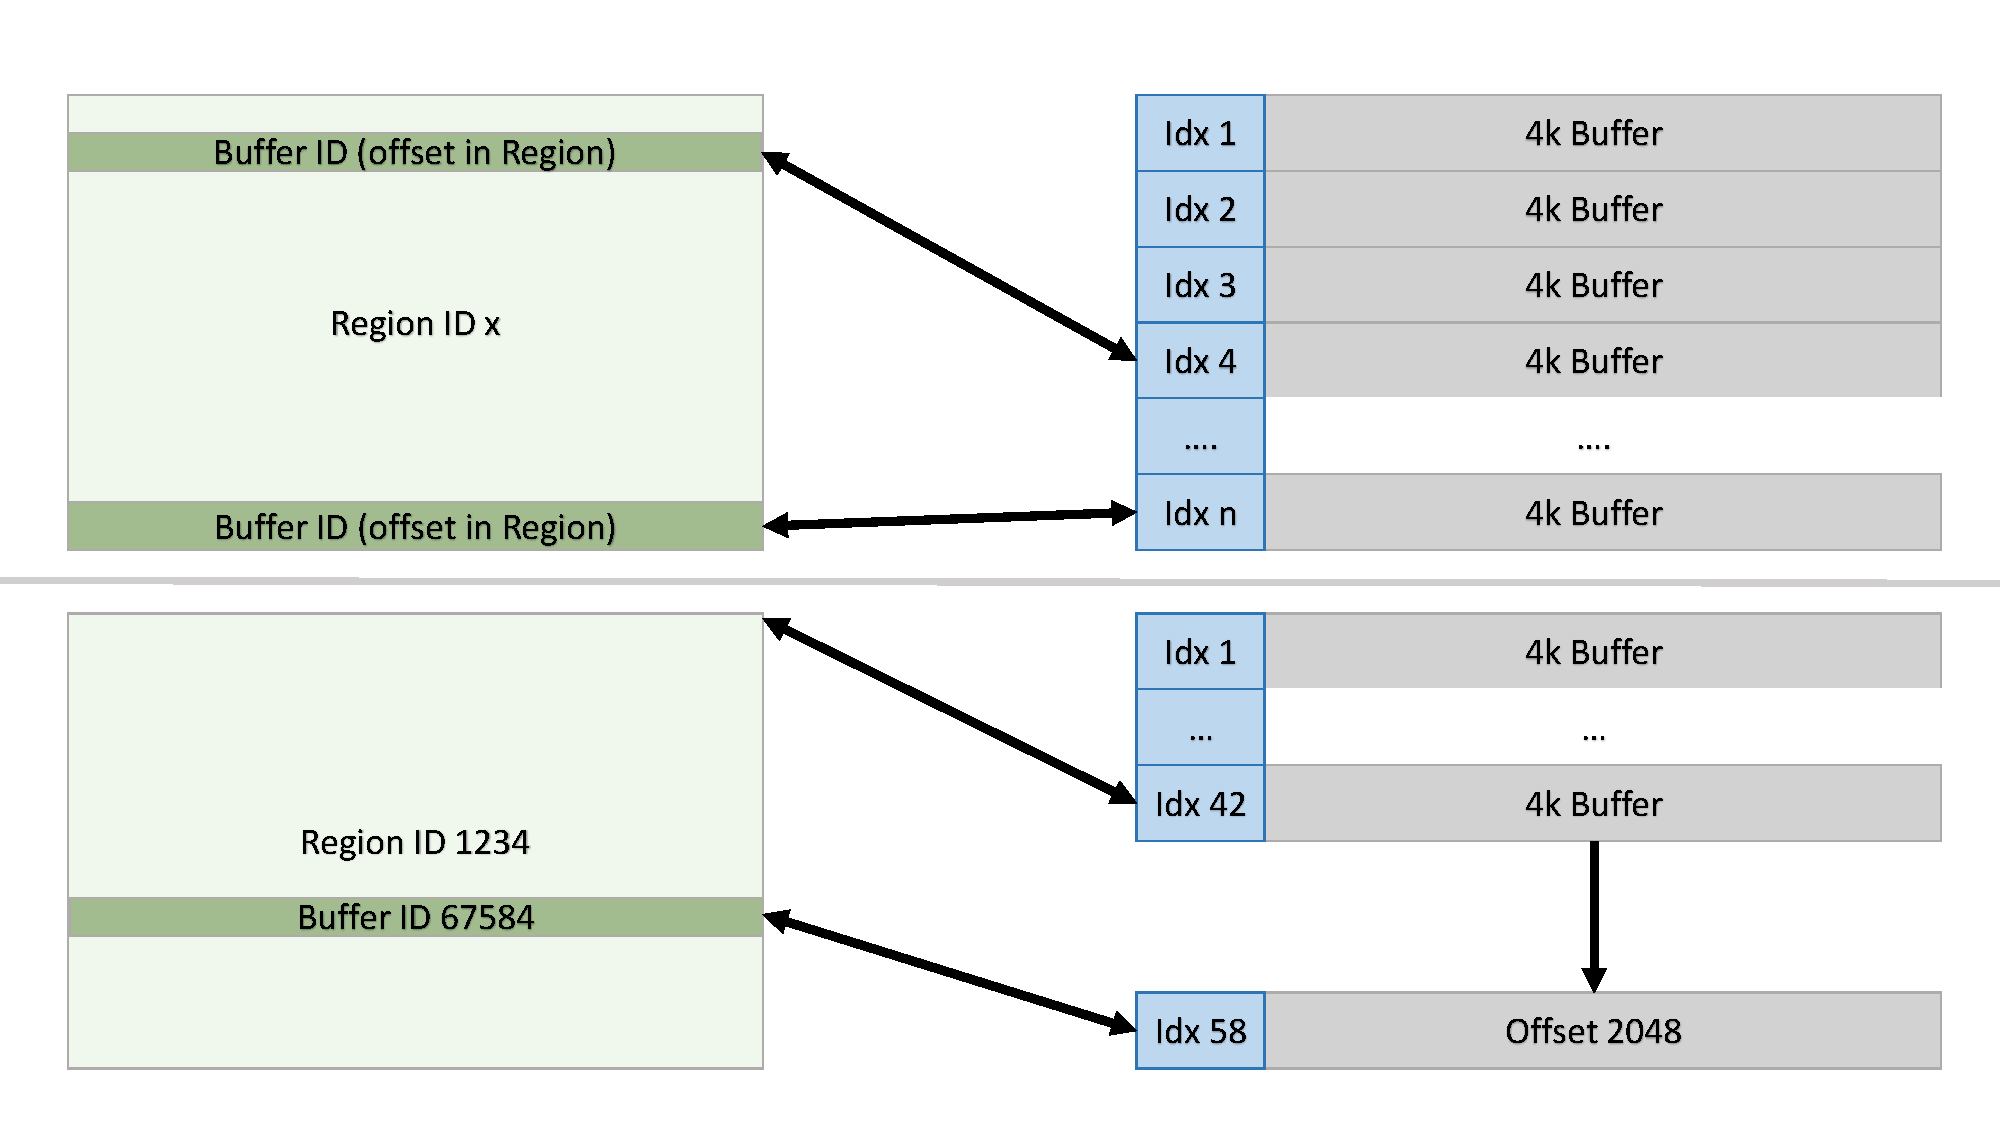
\includegraphics[width=\textwidth]{pics/sfn5122f.pdf}
	\label{fig:translation}
\end{figure}  

After the setup, we can directly access the hardware registers for managing the VNIC. If we call
\texttt{devq\_enqueue()} now, the region and buffer id are translated to an buffer table 
entry and an offset which can be used to build a descriptor. The \texttt{flags} of the 
\texttt{devq\_enqueue()} function are used to define if the buffer we enqueue is a receive 
or send buffer. Additionally to the descriptor, we also write the buffer id, region id and 
other information alongside the descriptor so a second translation of 
buffer table index to region and buffer id is not necessary on \texttt{devq\_dequeue()}. 
Since both \texttt{devq\_enqueue} and \texttt{devq\_dequeue} directly access hardware 
registers, \texttt{devq\_notify} is a NOP. Here we use the semantics, that enqueing/dequeueing 
on a queue is possible before receiving a notify.

\section{Implementation IDC Backend}
The IDC backend facilitates communication between two processes on either the same core
or two different cores. The communication channel is based on Flounder interfaces. To set 
up such a channel, one of the endpoints exports the interface while the other simply connects
to the endpoint that exports functionality. The flounder interfaces are shown in Figure \ref{lst:descq}.
\begin{figure}[h!]
	\caption{Flounder Interface}
	\begin{lstlisting}[style=code]
    interface descq "Devif communication queue" {
        // create and destroy a queue
        rpc create_queue(in uint32 slots, 
                         in cap rx, 
                         in cap tx,
	                     in bool notifications, 
                         out errval err);
                     
        rpc destroy_queue(out errval err);
	
        // add a memory region to the buffer table
        rpc register_region(in cap cap, 
                            in uint32 rid, 
                            out errval err);
                        
        rpc deregister_region(in uint32 rid, 
                              out errval err);
	
        rpc control(in uint64 cmd, 
                    in uint64 value, 
                    out errval err);
    
    };
	\end{lstlisting}
	\label{lst:descq}
\end{figure} 
On the remote side, the functions pointers that are given during creation are called. 
Using these function pointers, two queues can be connected (e.g. solaflare queue and 
IDC queue to support software filtering). If the endpoint simply 
connects to a remote endpoint, the local endpoint sets up memory for the receive/send 
queue that reside in shared memory between the two endpoints. 
The shared memory is established by the \texttt{create\_queue}
RPC call. There are no flounder RPC calls for enqueue and dequeue as they are handled through either 
a notification sent to the other endpoint or the remote endpoint can simply 
poll the queue by trying to dequeue a descriptor from the queue. 

\chapter{Interface Usage}
The usage in both cases, if the datapath is in a single domain or across domains is the same. 
In the case of a single domain, the notify can be dropped since it is a NOP. 
In a single domain the control plane, i.e. setting up the queue and registering memory 
regions to the interface, can involve another process but not on the data plane. 
In the following we make a small example of how to use the queue interface and
a queue backend. 
\begin{lstlisting}[style=code]
errval_t err;
struct queue* q;
struct descq* queue;
struct capref memory;
regionid_t regid;

// Create queue, specific to the queue backend. 
// In this case simple channel between two processes
err = descq_create(&queue, notify_cb, ...);
if (err_is_fail(err)){
    // error handling
}

// Cast to queue interface struct. Used for methods
// that are not 
q = (struct queue*) queue;

// Allocate memory (returns a capability to the memory)
err = frame_alloc(&memory, MEMORY_SIZE, NULL);
if (err_is_fail(err)){
    //error handling
}

// Register the memory we are going to use
err = queue_register(q, memory, &regid);
if (err_is_fail(err)){
    // error handling
}

\end{lstlisting}
At the point of the queue creation, we still have to know what the queue represents.
In this case we create a queue to connect two processes. Following the creation, we cast 
the device specific to a more general queue. Now, we can use the queue interface to register 
the memory from which we want to carve out our variable sized buffers. At this stage, the datapath
is set up and buffers can be transferred. 
\begin{lstlisting}[style=code]
// Modify buffers in some way
//  ...

// Enqueue buffers (2KB size for now, but can be variable size)
for (int i = 0; i < MEMORY_SIZE/2048; i++){
    err = queue_enqueue(q, regid_rx, i*2048, 2048, 0, 2048, 0);
    if (err_is_fail(err)){
        // Can do a notify if the queue is full
    
        if (err == QUEUE_ERR_QUEUE_FULL) {
            err = queue_notify(q);
            if (err_is_fail(err)) {
                // error handling
            }
            // there was an error i.e. retry enqueueing buffer
            i--;
        } else {
           // there was an error i.e. retry enqueueing buffer
           i--;
        }
    }
} 
\end{lstlisting}
In the example above, fixed sized buffers are enqueued and transferred to another process. 
The process on the other end of the queue can dequeue the buffers at any time but the queue
itself has a size limit (as many most other queues). When the other process does not dequeue
from the queue, at some point the queue will be full. As an optimization, the function \texttt{notify}
sends a message to the other process to inform it that there might be buffers in the queue. 
\\
The teardown of the queue is using the function \texttt{deregister} and \texttt{destroy}
\begin{lstlisting}[style=code]
// Make sure this process owns all the memory of the region
// ...

// Remove region from the active set
err = queue_deregister(q, regid, &memory);
if (err_is_fail(err)){
    // error handling
}

// Cleanup resources of the queue
err = queue_destroy(q);
if (err_is_fail(err)){
    // error handling
}
\end{lstlisting}
Before a region can be deregistered, the process has to make sure that all the memory of the region
is owned by the process. If the process does not fully own the region, \texttt{deregister} 
returns an error. Similar, \texttt{destroy} fails if there are still regions registered. 
\\
For the receiving part, the process simple has to dequeue from the queue
\begin{lstlisting}[style=code]
regionid_t rid;
genoffset_t offset;
genoffset_t length;
genoffset_t valid_data;
genoffset_t valid_length;
uint64_t flags;

err = queue_dequeue(q, &rid, &offset, &length, &valid_data, &valid_length, &flags);
if (err_is_fail(err)) {
    //error handling, 
}
\end{lstlisting}
Additionally in the case of the queue for inter process communication during creation
a notification handler can be given as an argument. An example of such a handler is shown below.
This handler is called whenever a \texttt{notify} from the other process is received. 
\begin{lstlisting}[style=code]
static void notify_cb(void* q)
{
    errval_t err = SYS_ERR_OK;
    struct queue* queue = (struct queue*) q;

    regionid_t rid;
    genoffset_t offset;
    genoffset_t length;
    genoffset_t valid_data;
    genoffset_t valid_length;
    uint64_t flags;

    while(err_is_ok(err)) {
        err = queue_dequeue(queue, &rid, &offset, &length, &valid_data,
                            &valid_length, &flags);
    }
}
\end{lstlisting}
Some other examples are shown in Figures \ref{fig:oneproc} and \ref{fig:twoproc}
\begin{figure}[!h]
	\begin{center}
		\caption{Usage example with datapath in a single domain}
		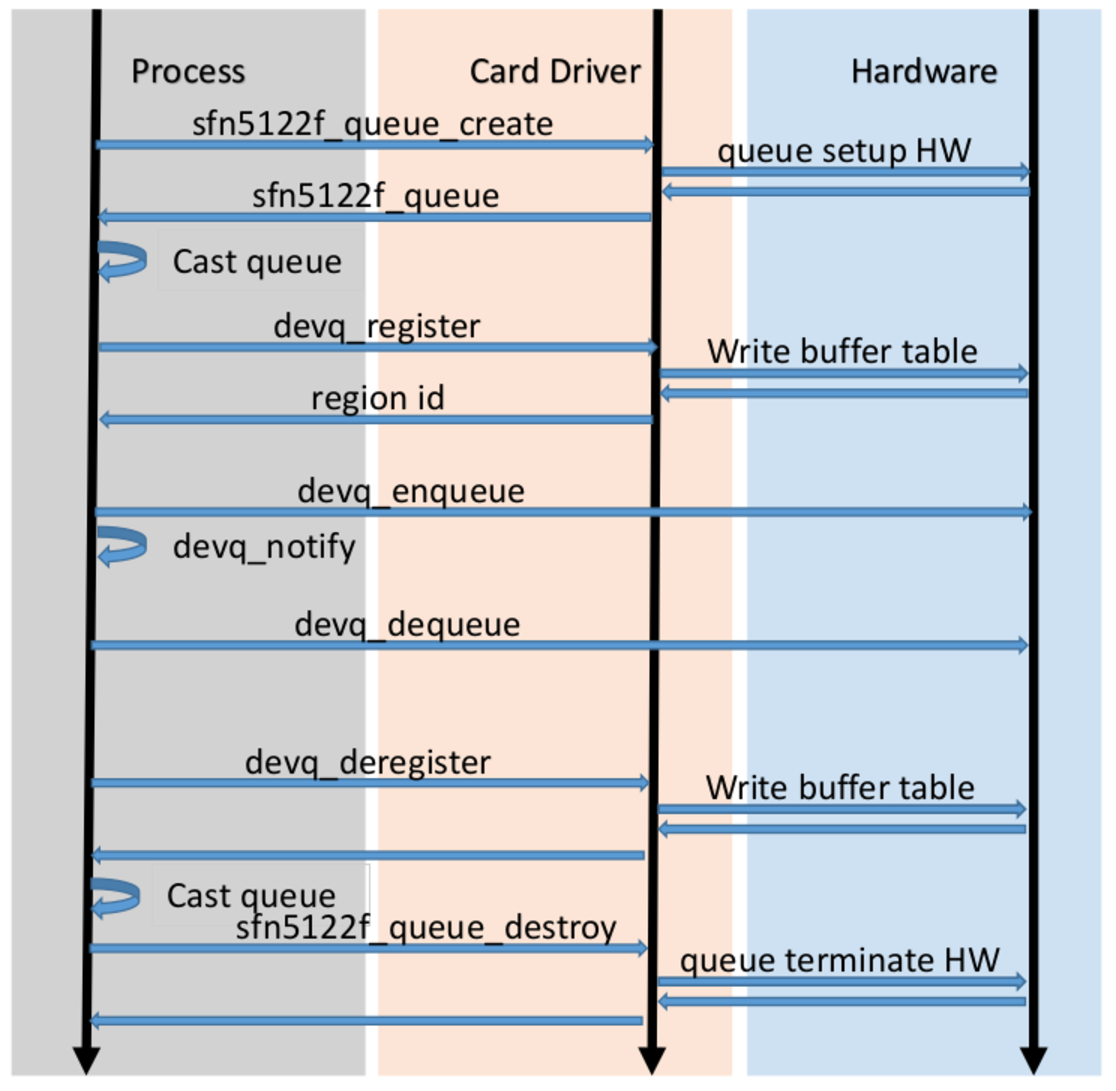
\includegraphics[width=0.65\textwidth]{pics/oneproc.pdf}
		\label{fig:oneproc}
	\end{center}
\end{figure}

\begin{figure}[!h]
	\begin{center}
		\caption{Usage example with datapath across domains}
		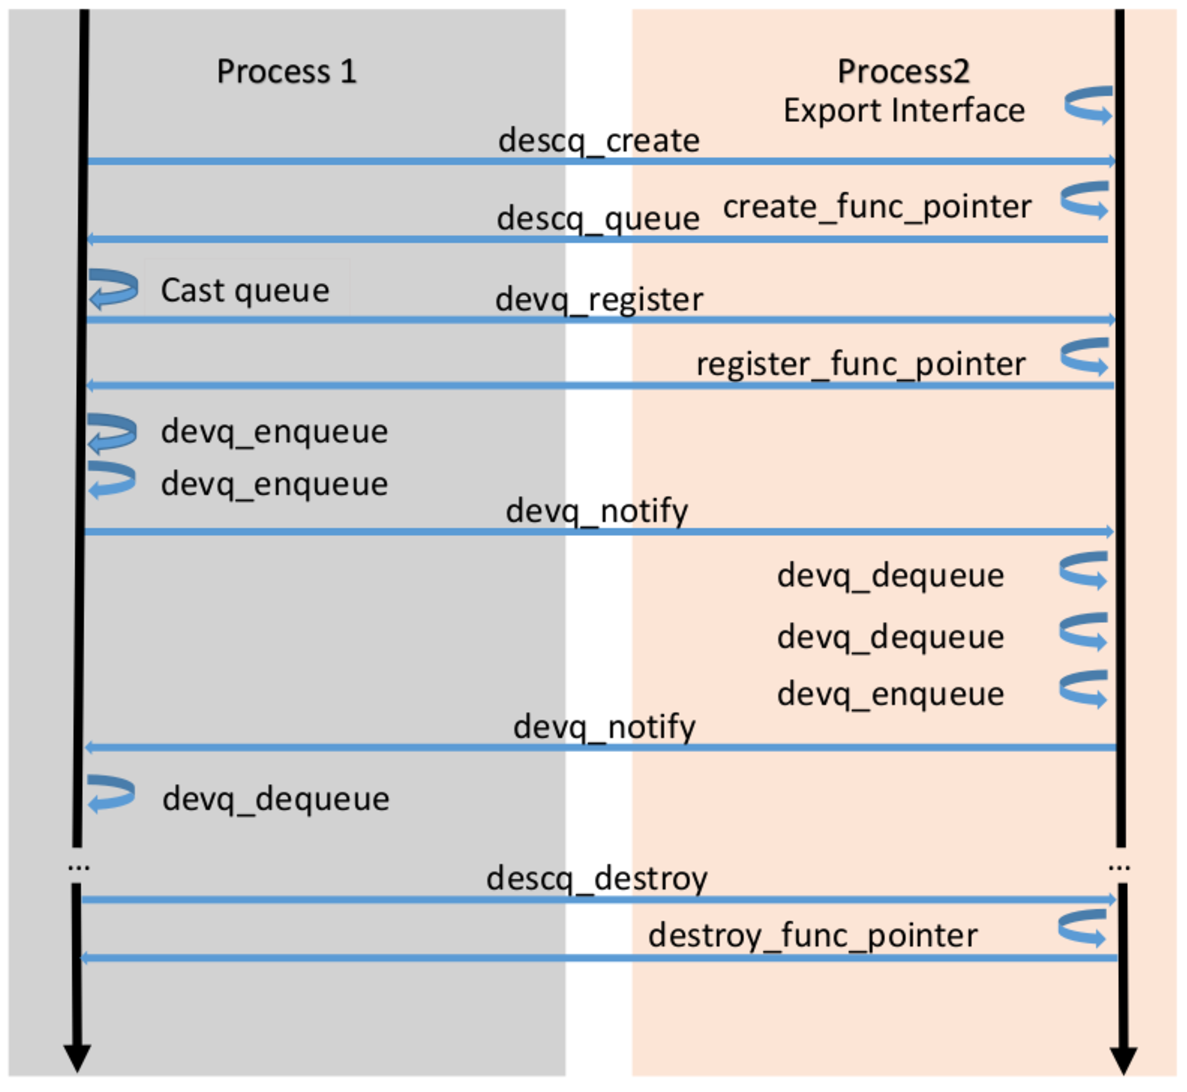
\includegraphics[width=0.65\textwidth]{pics/twoproc.pdf}
		\label{fig:twoproc}
	\end{center}
\end{figure}


\bibliographystyle{abbrv}
\bibliography{defs,barrelfish}	
	
\end{document}
